\newgeometry{top=2.5cm, bottom=0cm, left=4cm, right=2cm, nofoot}
\setcounter{table}{0}

\chapter{Havaintoja analyyttien käyttäytymisestä}\label{appx:havainnot}
\vspace{-24pt}
\section{Alluranpunainen}
%\vspace{-24pt}
ESI- puolella \textit{alluranpunaisen} Q1 (451,2 > 371,1) viereen ilmestyy ajan myötä toinen piikki retentiolla 4,40. \textit{Alluranpunaisen} hajoamistuote tämä ei voi olla, koska alkuperäinen piikki ($t_R$ 3,83) sijoittuu kalibrointisuoralle mainiosti. Kyseessä on luultavasti jonkin toisen analyytin hajoamistuote.
\begin{figure}[!htbp]
  \centering
    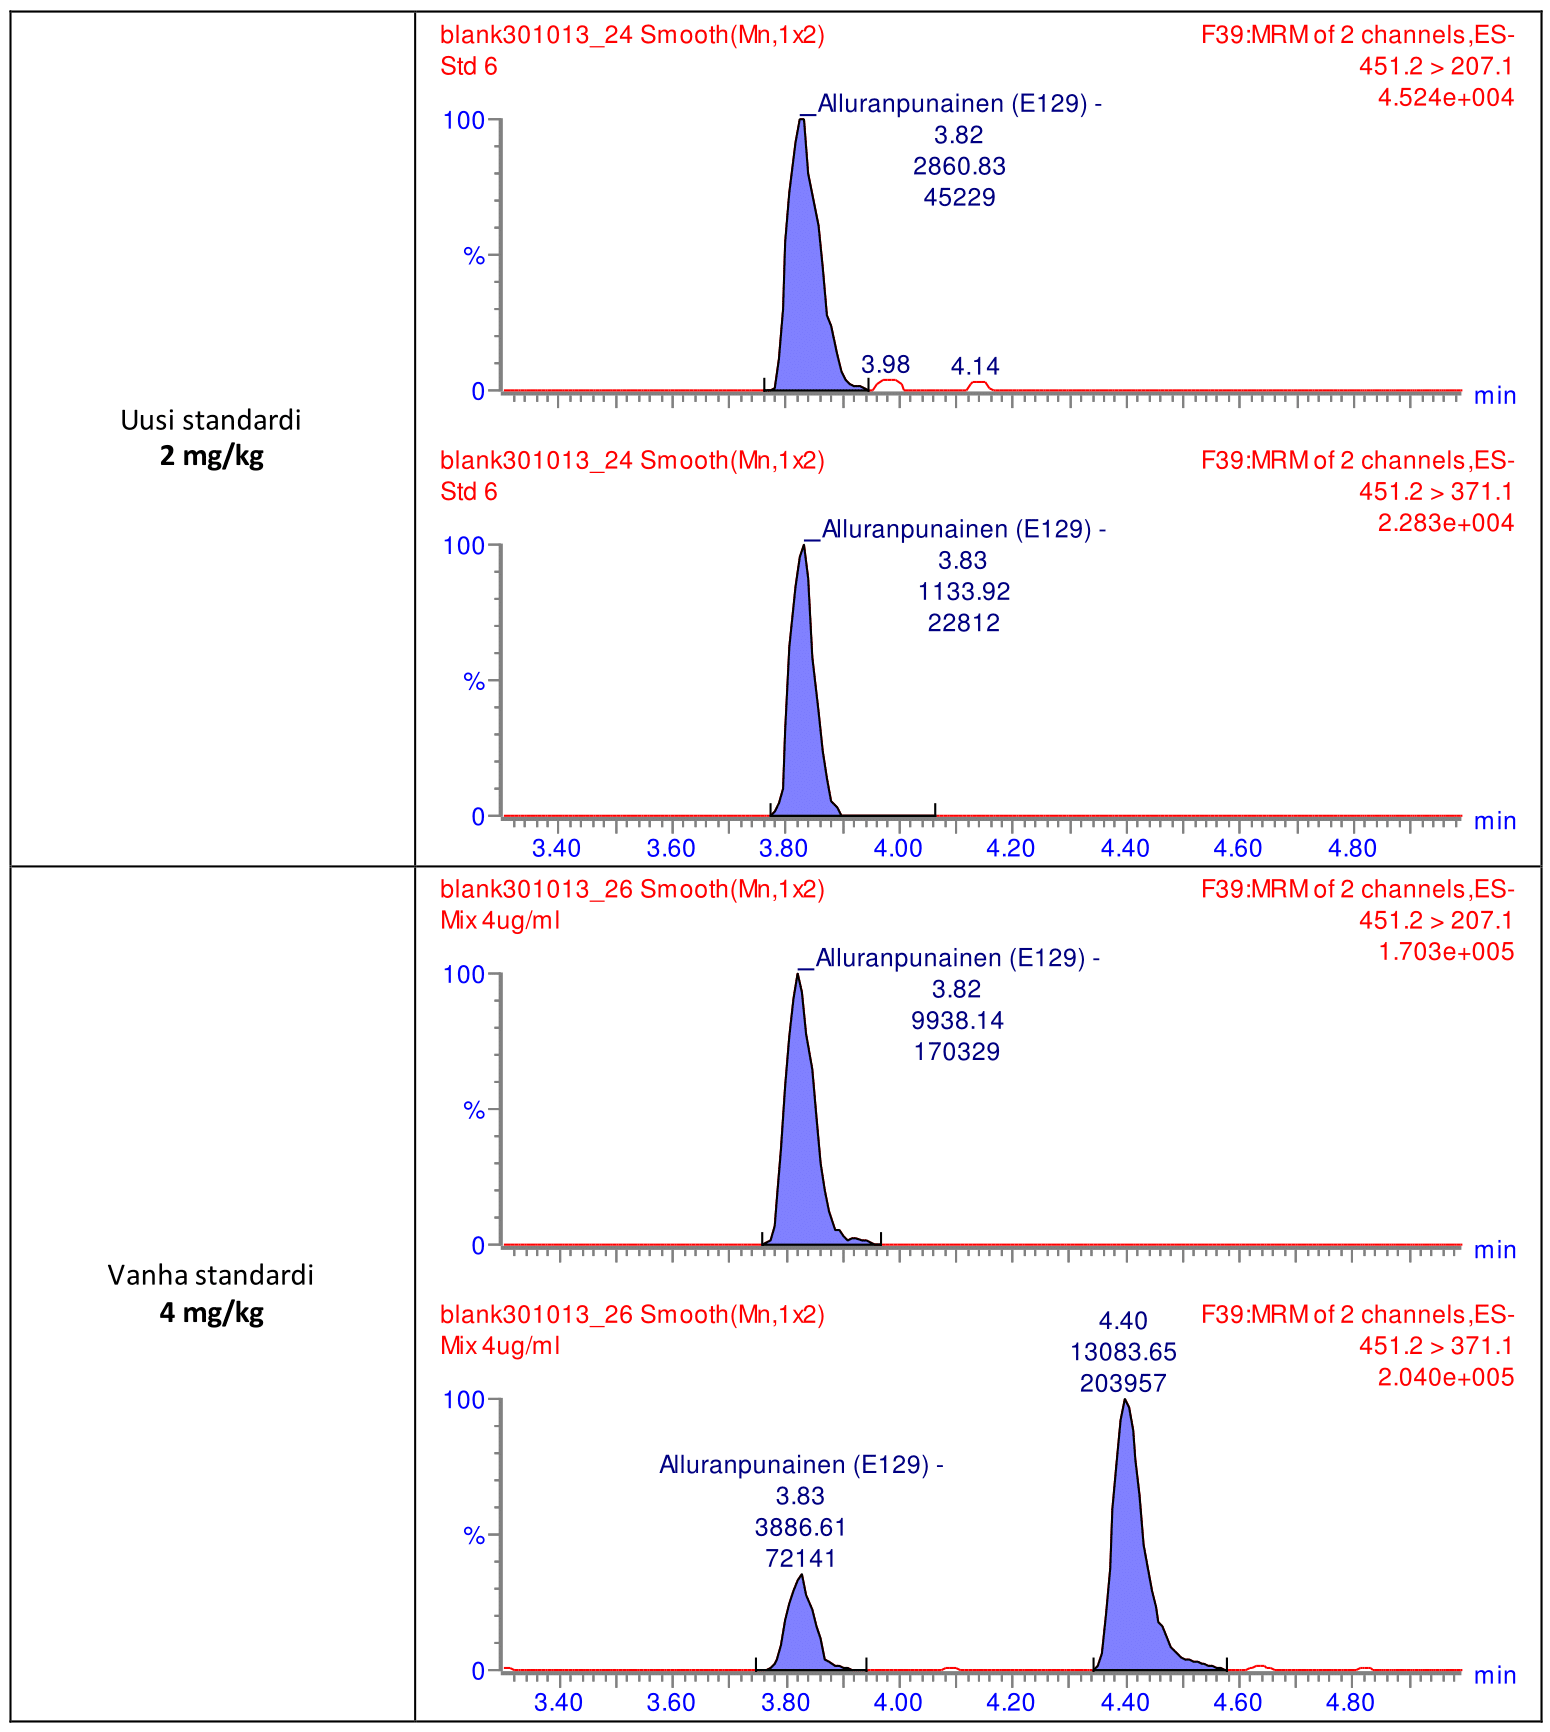
\includegraphics[width=\textwidth]{info-01}
\end{figure}
\clearpage
\section{Amarantti ja Uuskokkiini}
Identtinen retentioaika sekä pilkkoutuminen eli näitä kahta väriainetta ei pystytä erottamaan tällä menetelmällä. Esimerkkinä näyte, josta löydettiin TLC-menetelmällä vain \textit{uuskokkiini}.
\begin{figure}[!htbp]
  \centering
    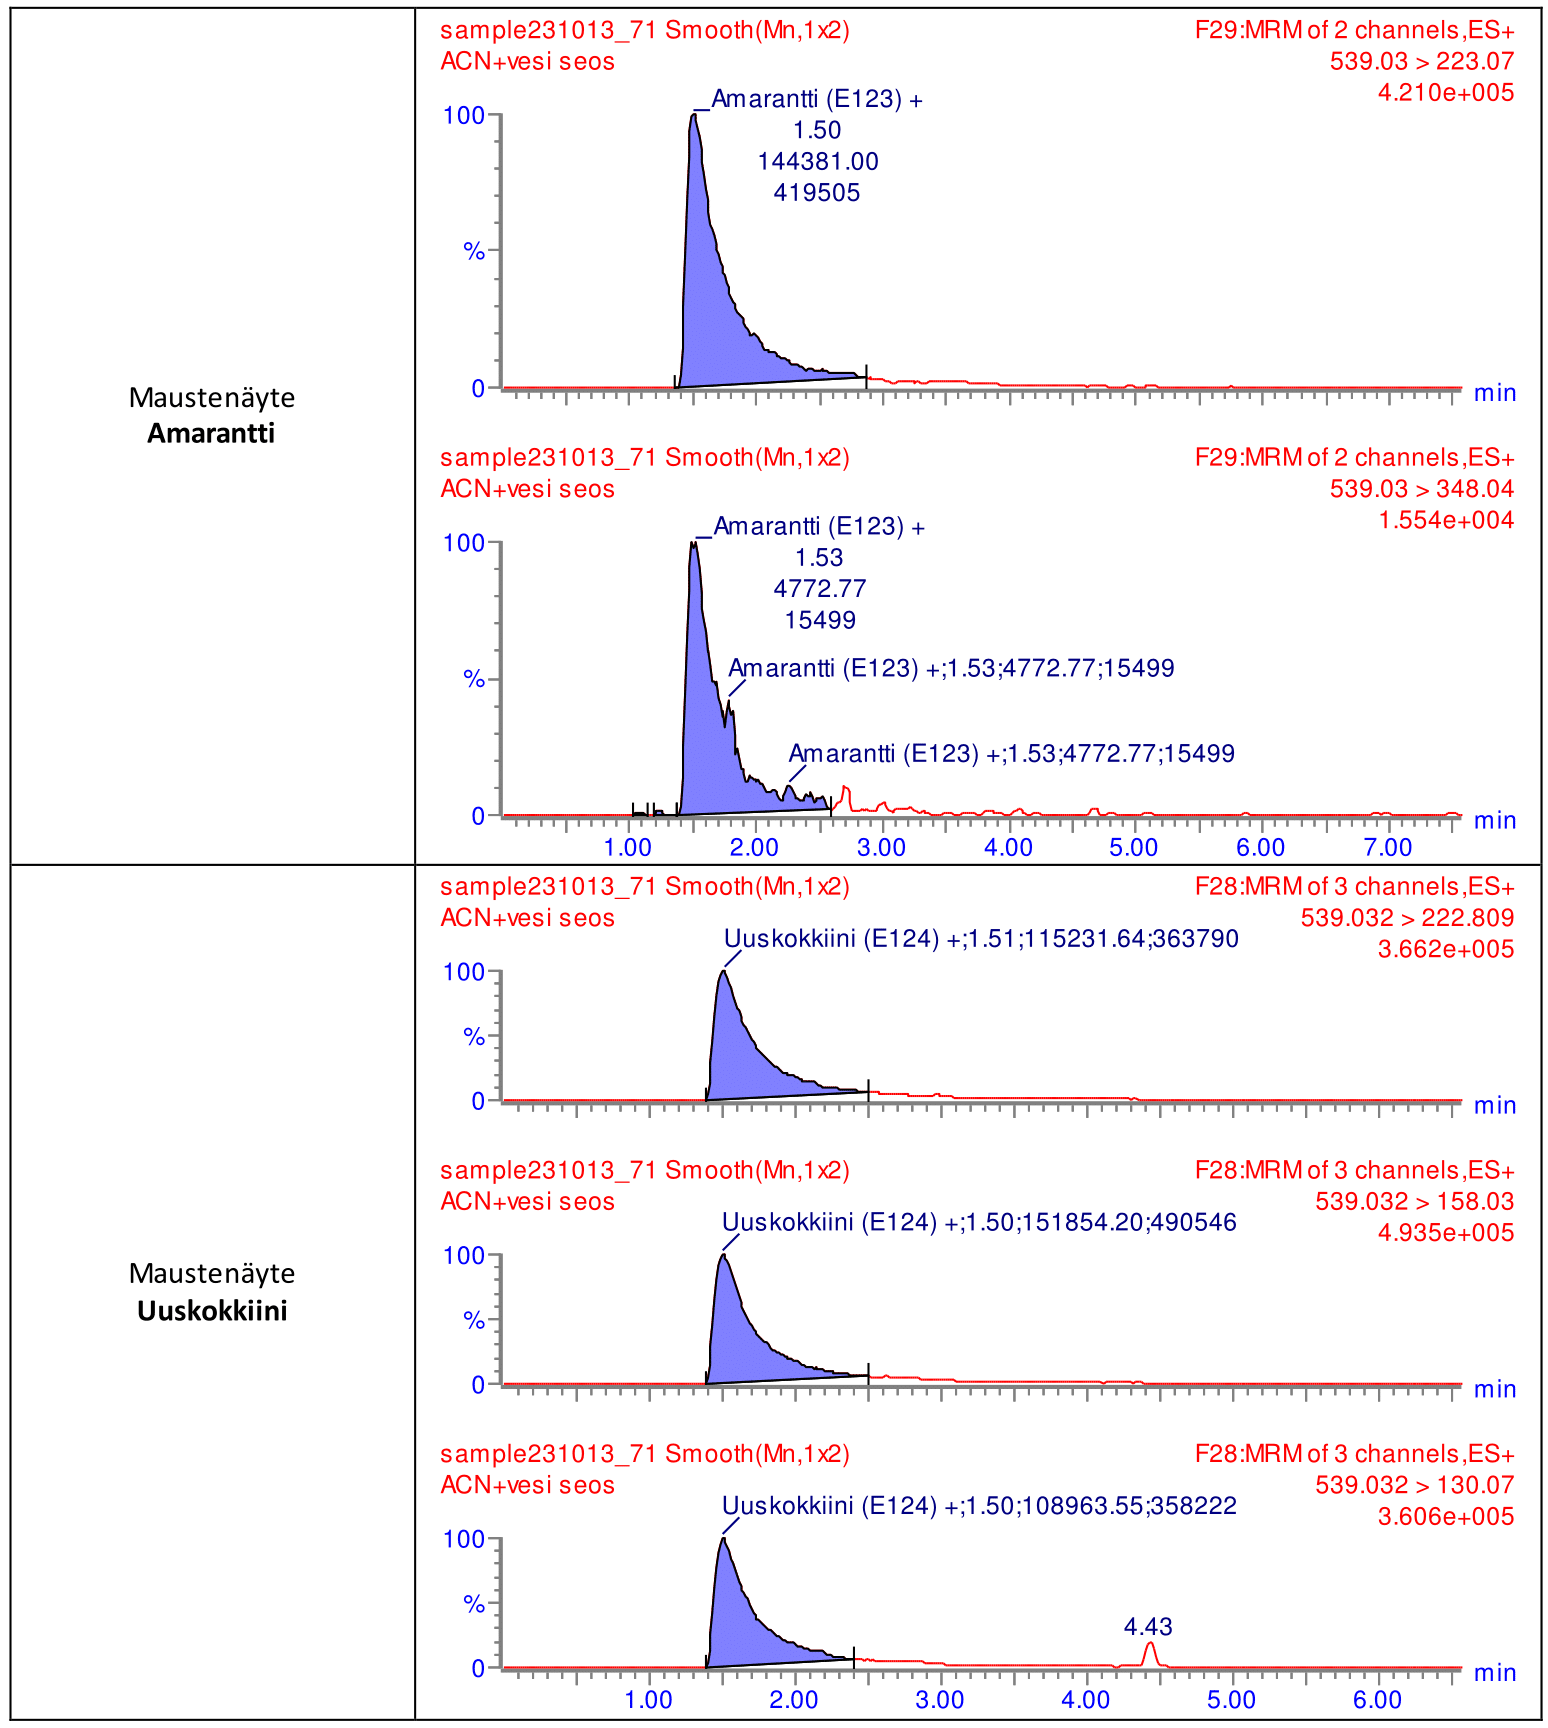
\includegraphics[width=\textwidth]{info-02}
\end{figure}
\clearpage
\section{Briljanttimusta}
\textit{Briljanttimustan} alkuperäiset MS-parametrit eivät olleet toimivat. \textit{Briljanttimustalle} yritettiin etsiä manuaalisesti syöttämällä puhdasta standardia suoraan massaspektrometrille. Briljanttimustalle löydettiin uudet parametrit negatiiviselta (ESI-) puolelta, joita kokeiltiin ajamalla puhdas standardi. Kuvassa on kyseisen ajon kromatogrammi, josta nähdään etteivät löydetyt parametrit ole kovin optimaaliset.
\begin{figure}[!htbp]
  \centering
    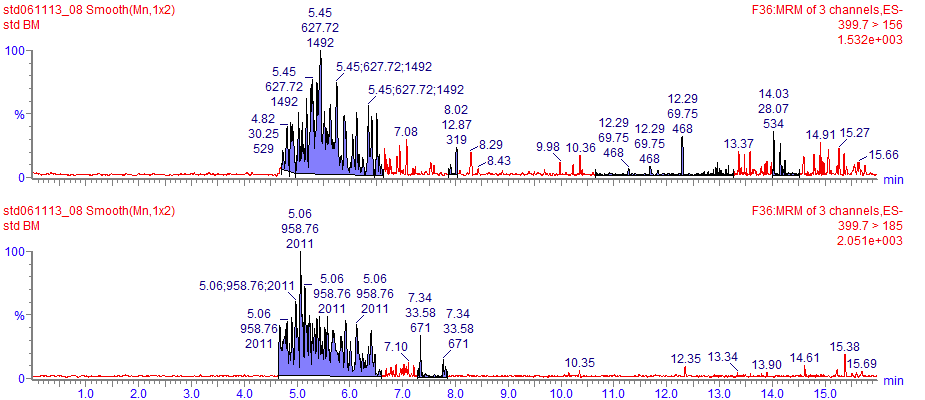
\includegraphics[width=\textwidth]{briljantti}
\end{figure}
\clearpage
\section{Fast Green FCF}
\textit{Fast green fcf:n} Q2:lla (764,71 > 169,71) on eri retentioaika verrattuna targettiin ja Q1:een. Tämä mahdollisesti johtuu standardin sisältämästä useasta eri analyytistä. Puhdasaineena Q2:n retentioaika olisi todennäköisesti sama.
\begin{figure}[!htbp]
  \centering
    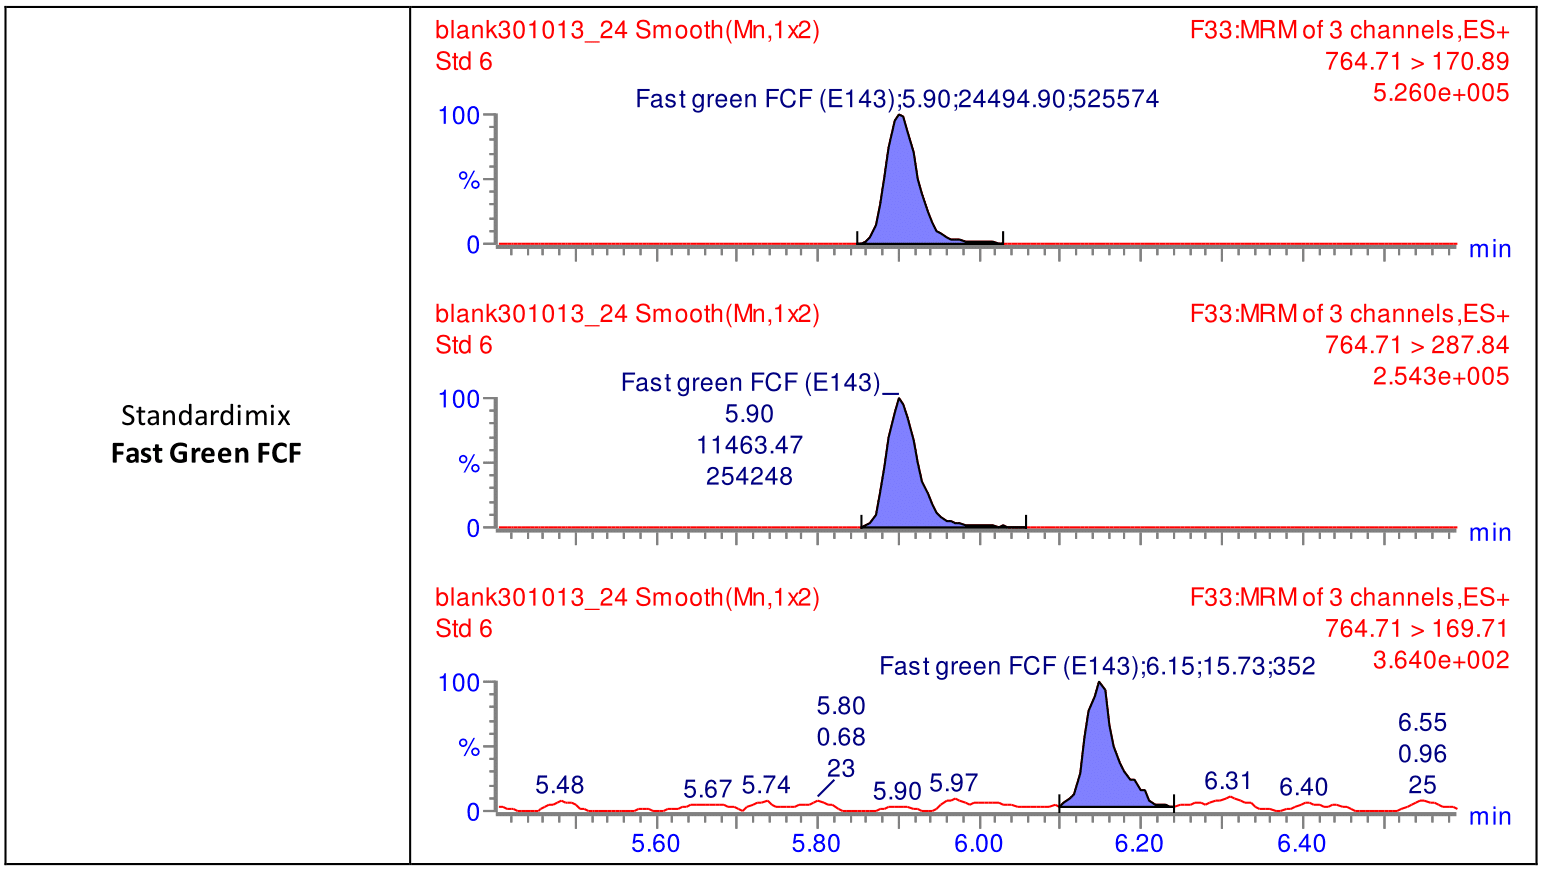
\includegraphics[width=\textwidth]{info-03}
\end{figure}
\clearpage
\section{Karmosiini}
\textit{Karmosiinin} Q1:llä eri retentioaika negatiivisella puolella standardimixissä kuin puhtaana aineena tai Q1:n vaste on todella pieni.
\begin{figure}[!htbp]
  \centering
    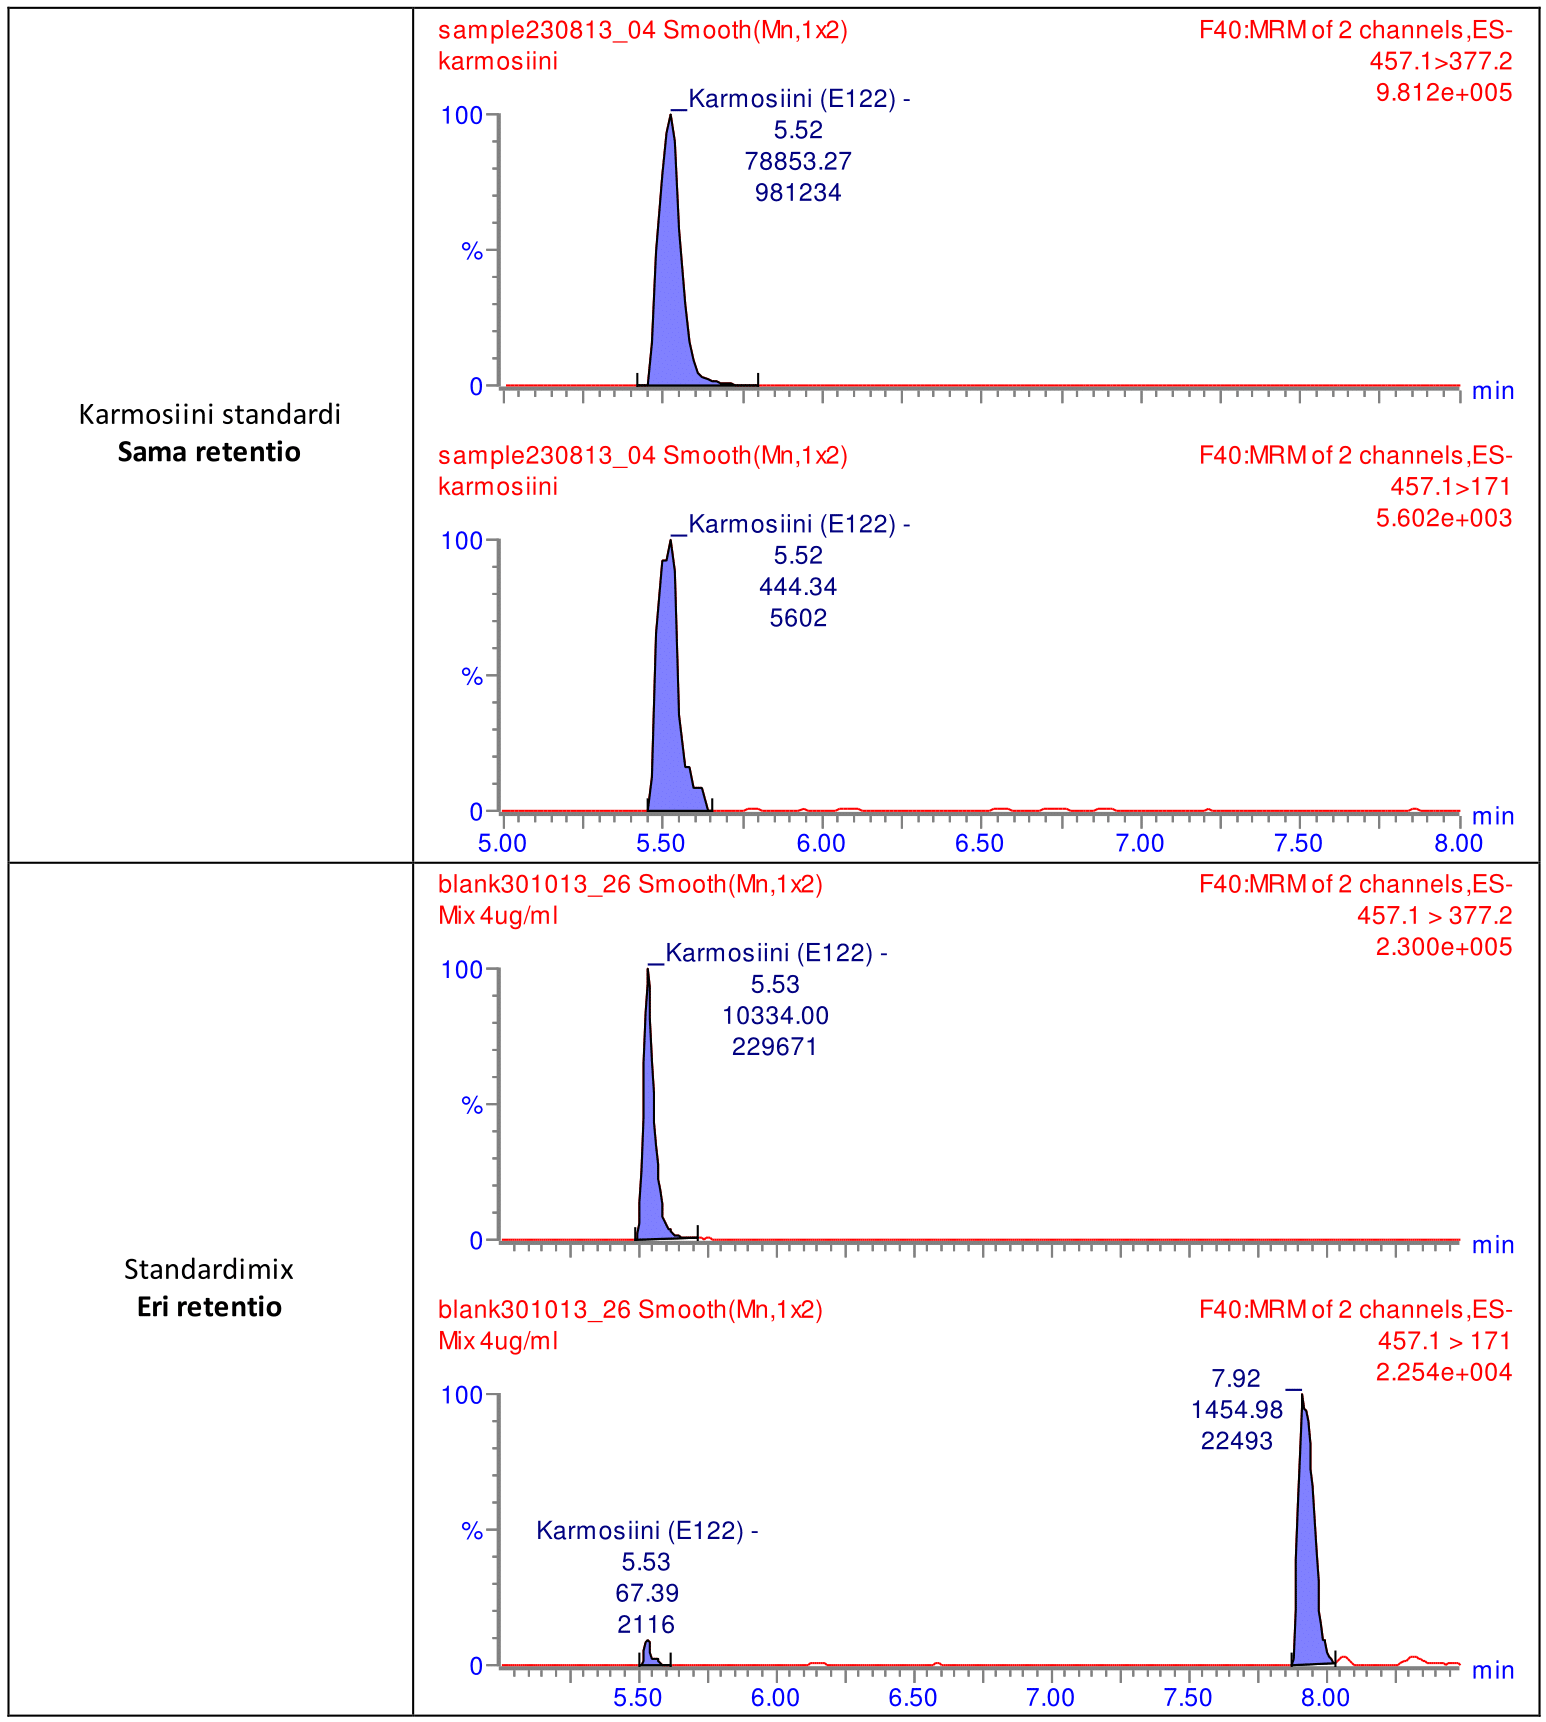
\includegraphics[width=\textwidth]{info-04}
\end{figure}
\clearpage
\section{Kurkumiini}
\textit{Kurkumiini} hajoaa ajan myötä. Uusi piikki on mahdollisesti \textit{kurkumiinin} isomeeri.
\begin{figure}[!htbp]
  \centering
    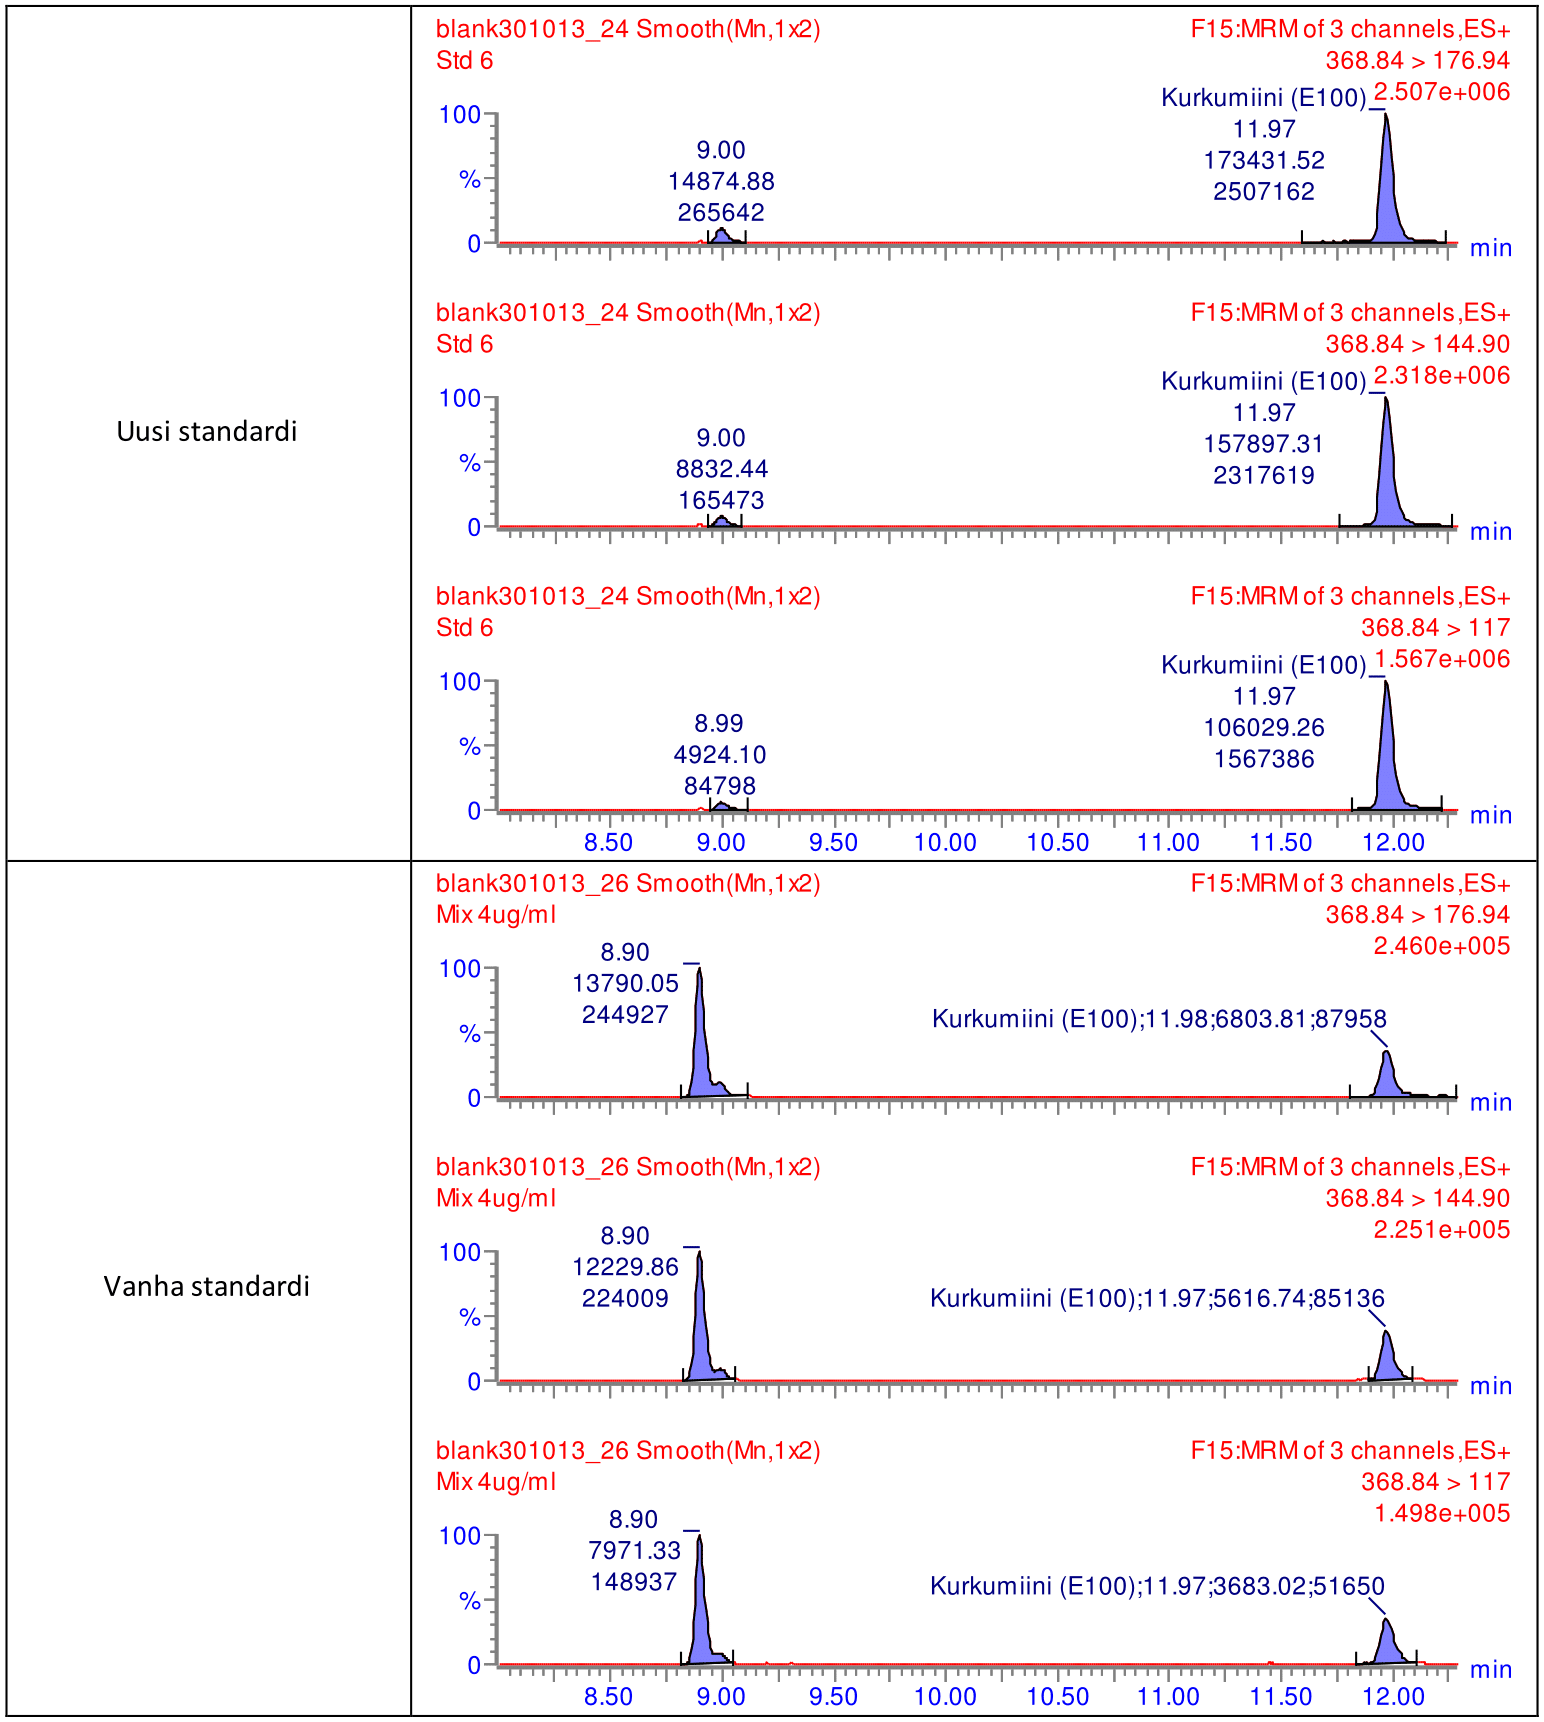
\includegraphics[width=\textwidth]{info-05}
\end{figure}
\clearpage
\section{Paraoranssi}
Tarkemmalla tutkinnalla \textit{paraoranssi} standardi sisältää kiellettyä \textit{orange II} väriainetta. Tämä todettiin yksittäisellä \textit{paraoranssi}standardilla, jonka pitoisuus oli 1 mg/kg.
\begin{figure}[!htbp]
  \centering
    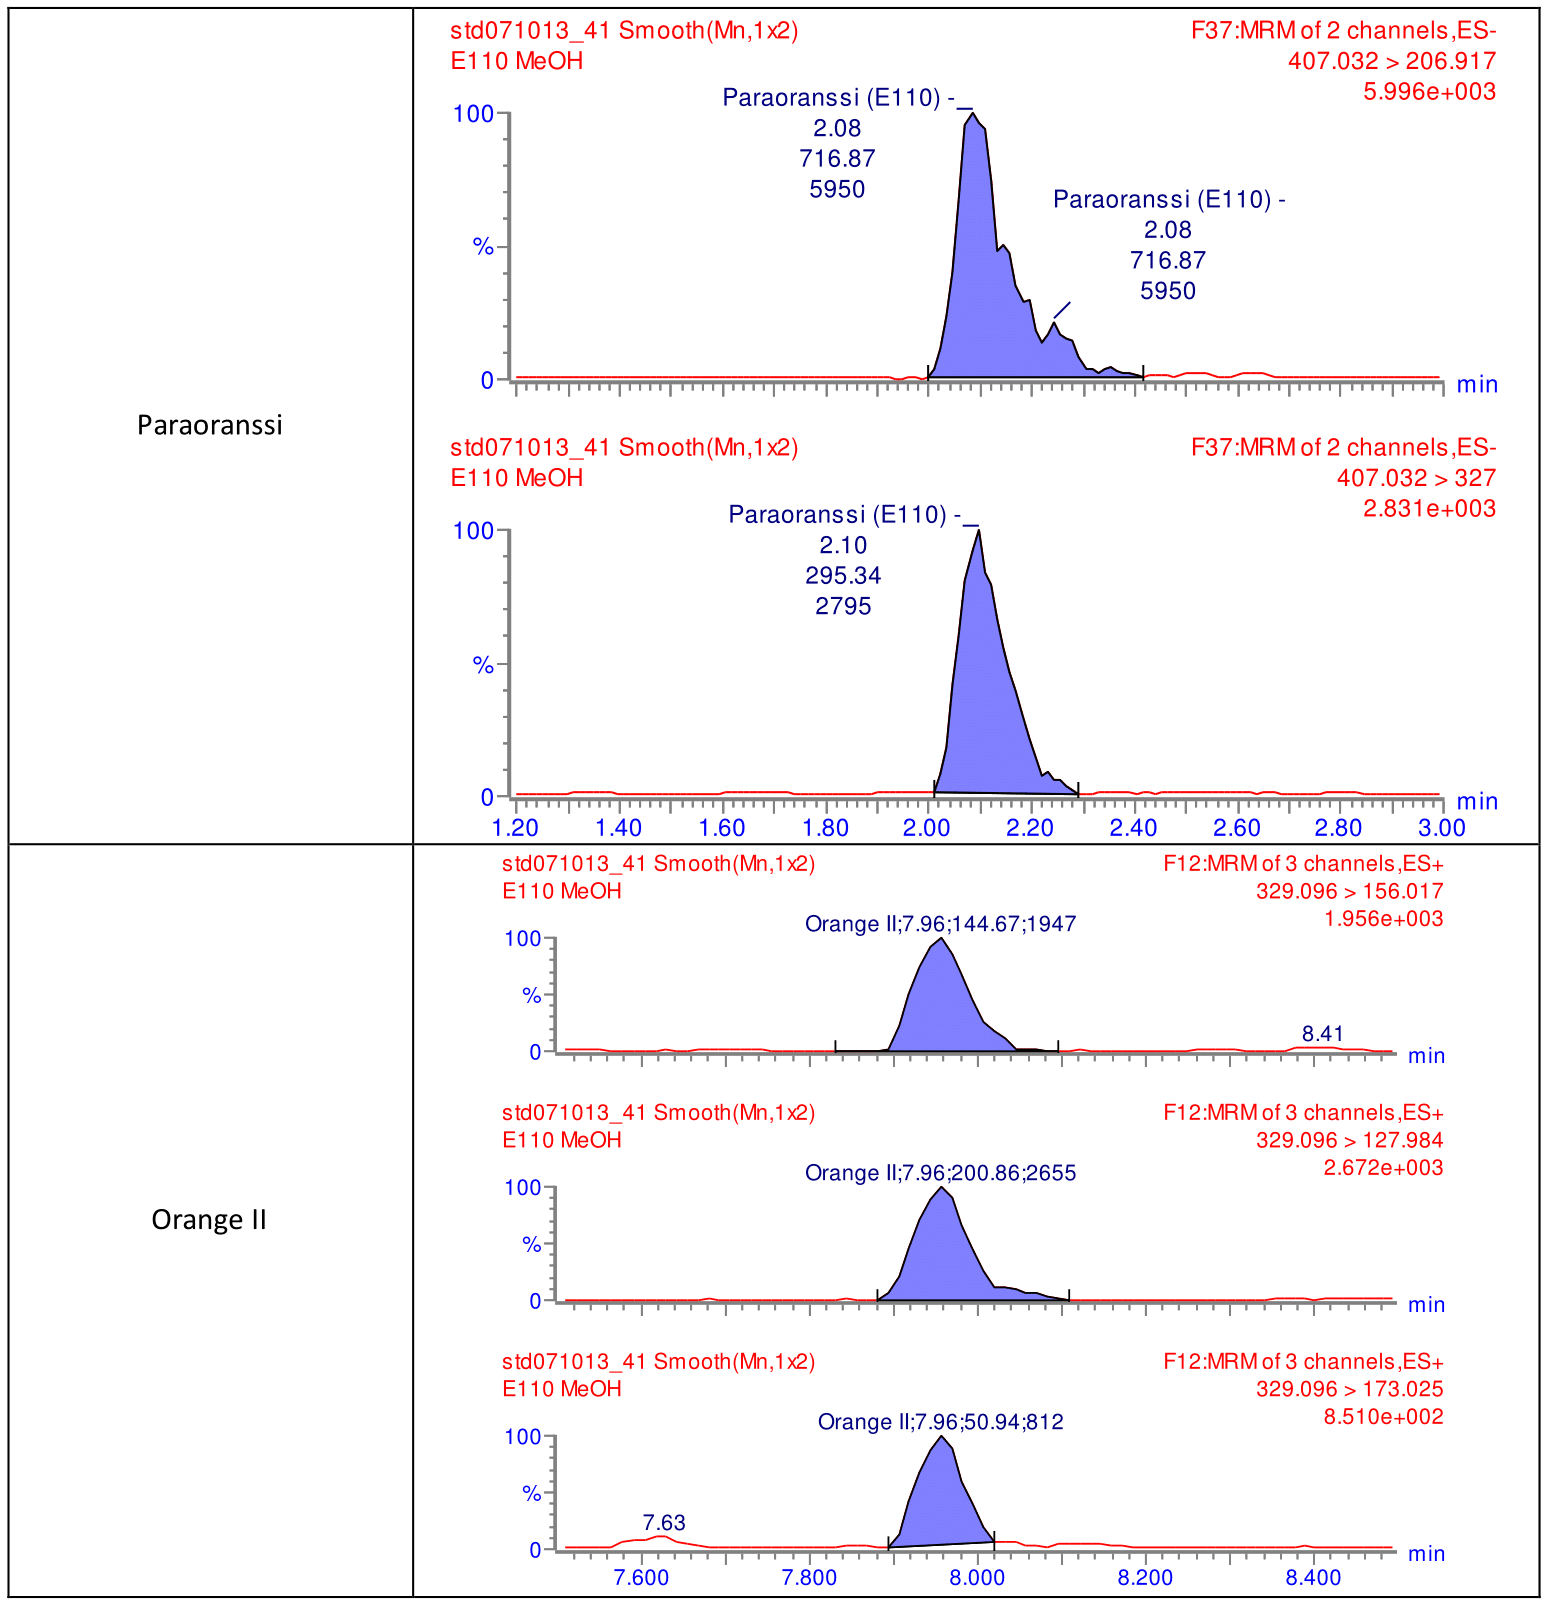
\includegraphics[width=\textwidth]{info-10}
\end{figure}
\clearpage
\section{Ruskea HT}
\textit{Ruskea ht:n} kohdalla tehtiin samoin kuin \textit{briljanttimustalle}. \textit{Ruskea ht:lle} saatiin uudet lupaavat MS-parametrit, joiden avulla saatiin tehtyä standardisuora. Tätä kokeilua pidemmälle ei ehditty päästä.
\begin{figure}[!htbp]
  \centering
    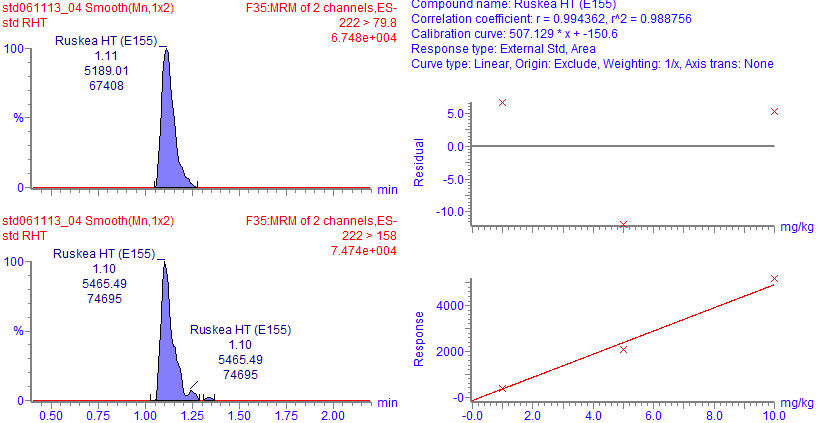
\includegraphics[width=\textwidth]{rht}
\end{figure}
\clearpage
\section{Sudan IV ja Sudan red B}
Analyyttien erottuminen huono, lähes sama retentioaika. Ilmenee tuplapiikkinä standardimixissä. Puhdasaineina saattaisi erottua toisistaan.
\begin{figure}[!htbp]
  \centering
    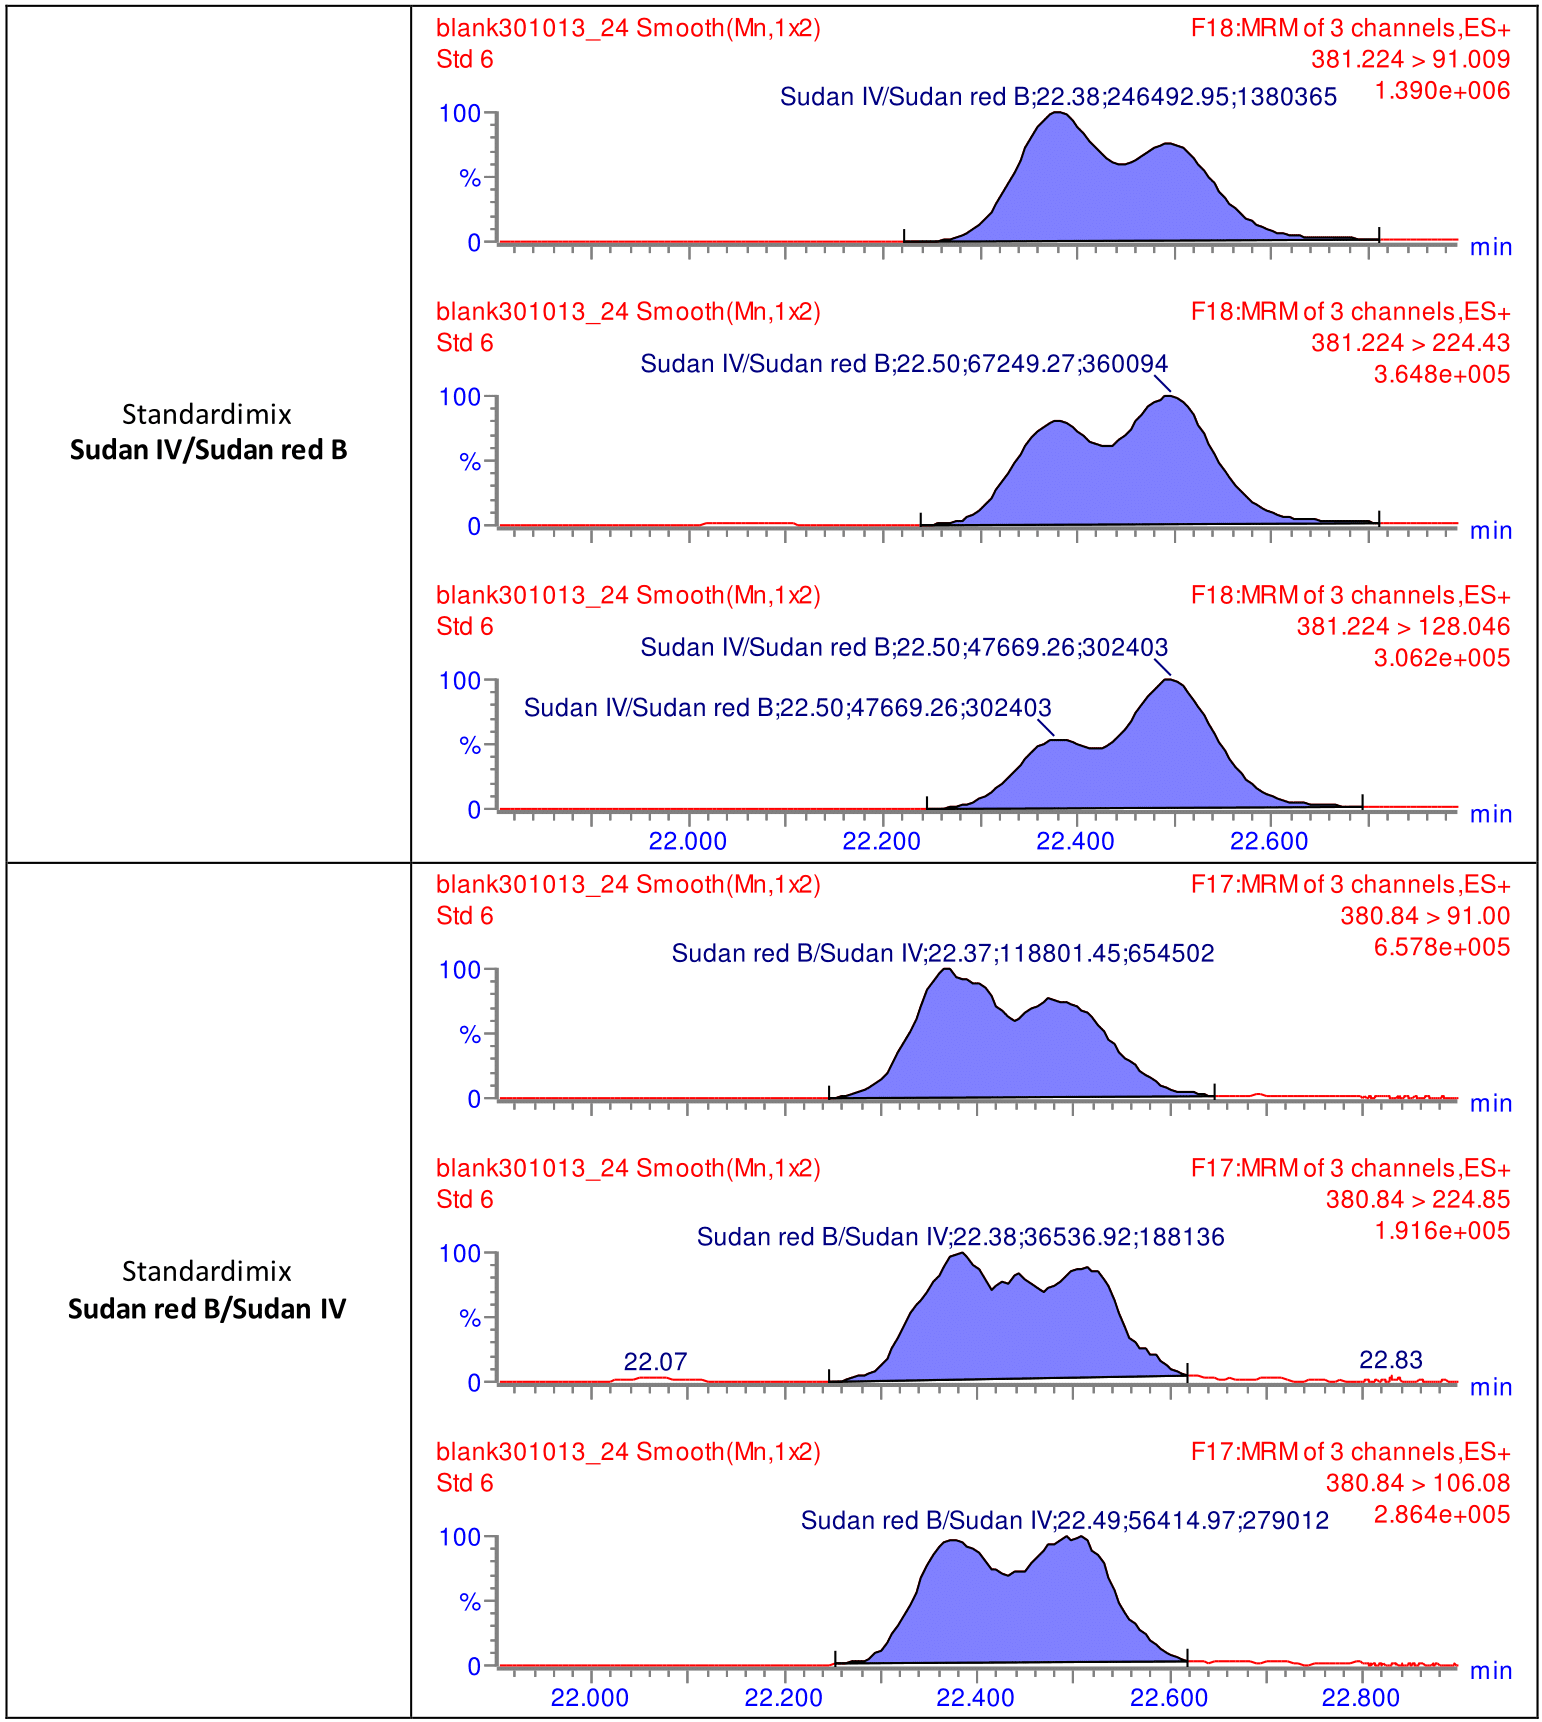
\includegraphics[width=\textwidth]{info-06}
\end{figure}
\begin{figure}[!htbp]
  \centering
    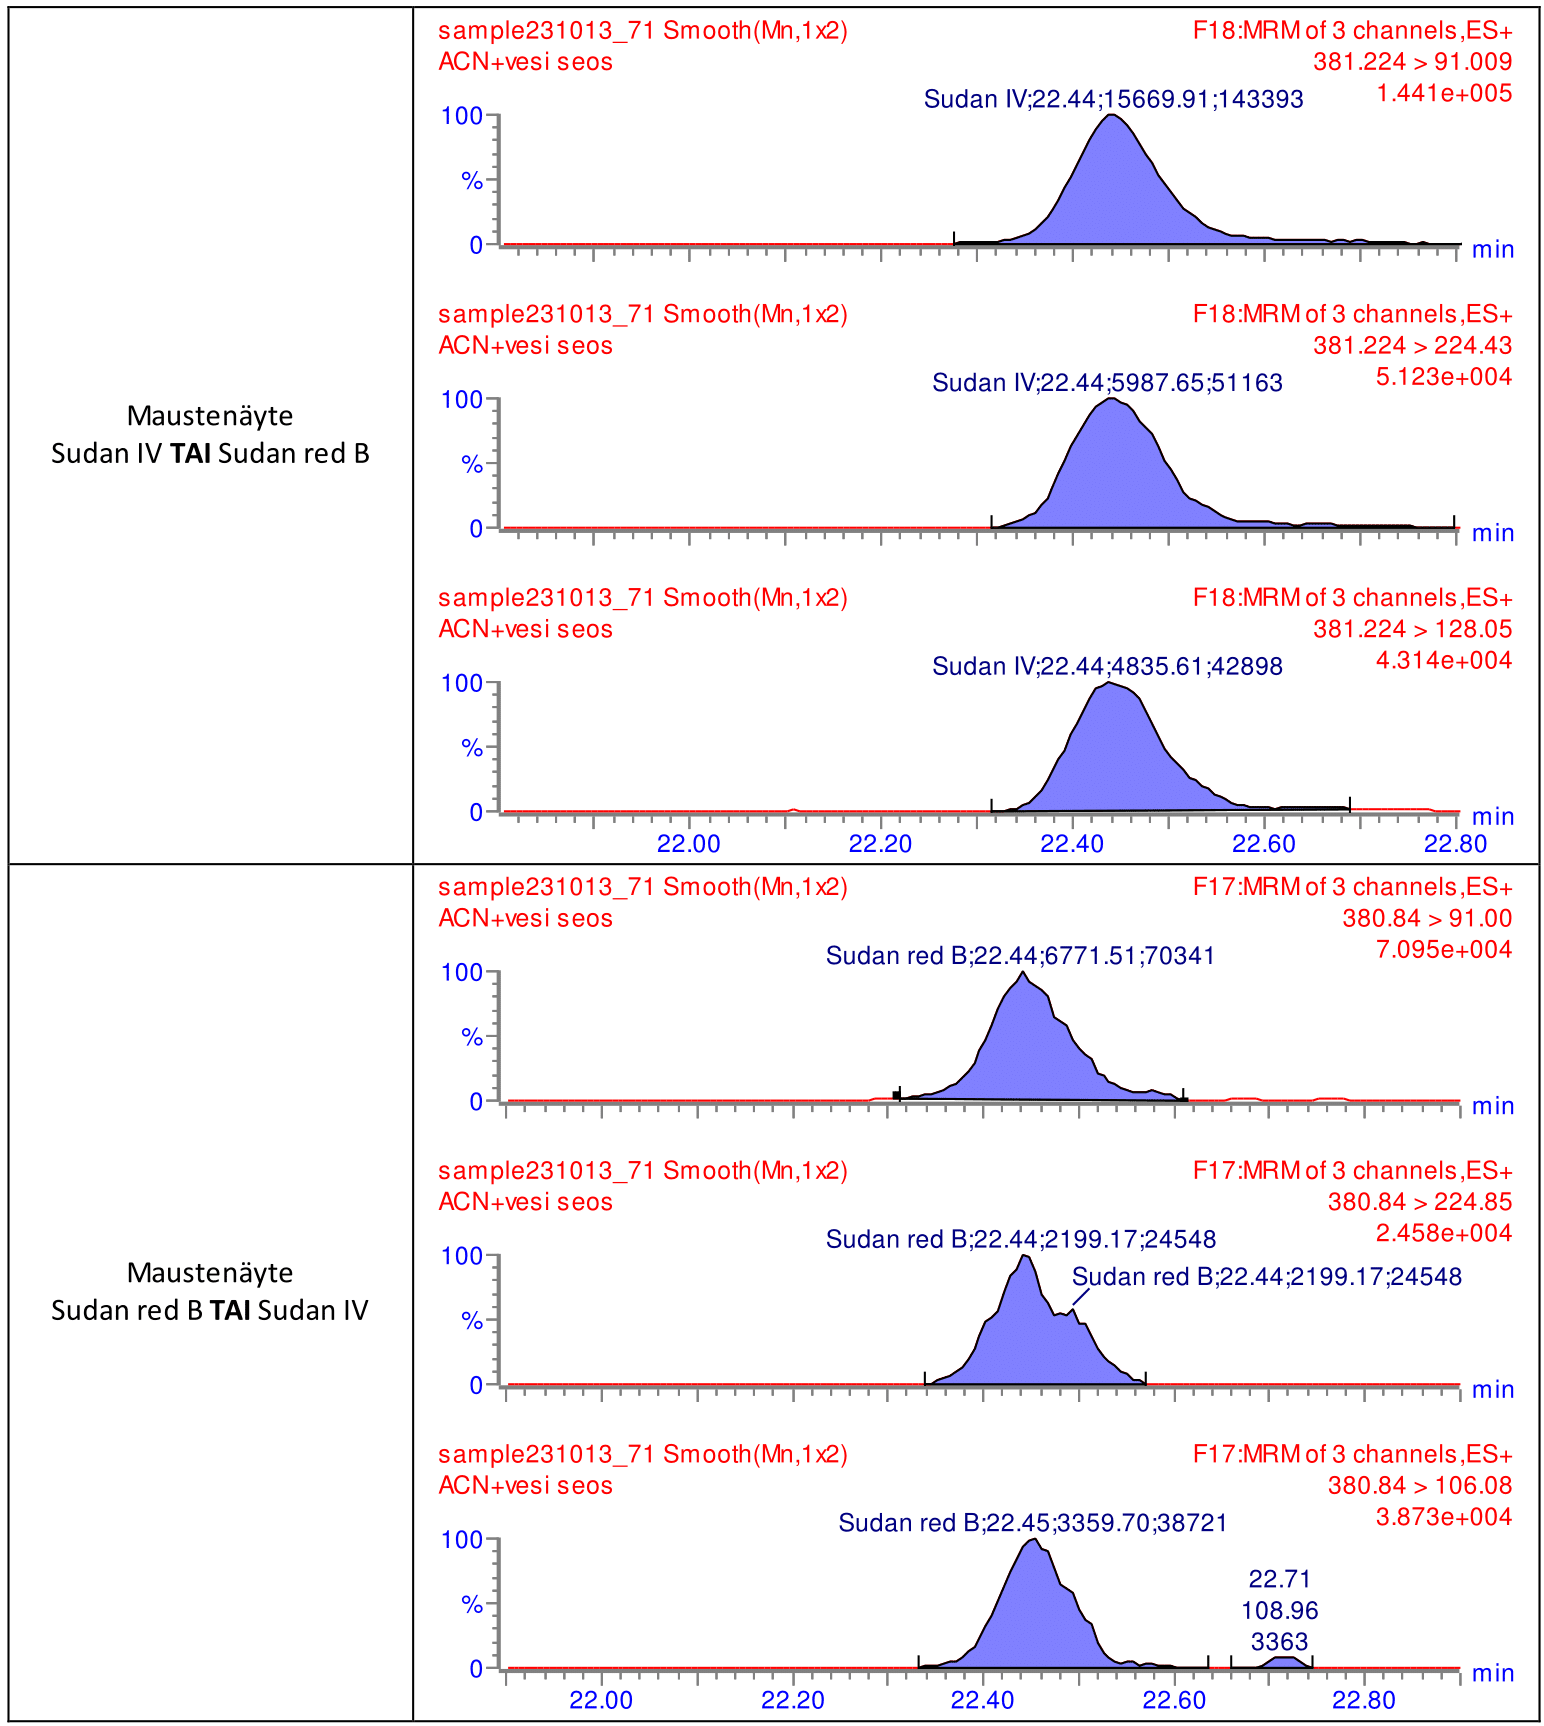
\includegraphics[width=\textwidth]{info-07}
\end{figure}
\clearpage
\section{Todella suuren vasteen analyytit}
\vspace{-24pt}
Suuren vasteen antava analyytti saattaa näkyä toisen analyytin kromatogrammissa ylimääräisenä piikkinä. Esimerkkinä \textit{kurkumiini} ($t_R$ 11,96) näkyy suuressa pitoisuudessa sekä \textit{erytrosiinin} ($t_R$ 11,58) sekä \textit{rhodamine b:n} ($t_R$ 12,34) kromatogrammeissa suurena piikkinä.
\begin{table}[!htbp]
  \centering
  \caption{Häiritseviä analyyttejä ja niiden $t_R$}
    \begin{tabular}{lr}
    \toprule
    Analyytti & Retentioaika (min)\\
    \midrule
    Patenttisininen & 8,31 \\
    Kurkumiini & 11,96 \\
    Rhodamine B & 12,34 \\
    Fast Garnet GBC & 14,07 \\
    \bottomrule
    \end{tabular}%
  \label{tab:suurianalyytti}%
\end{table}%
\begin{figure}[!h]
  \centering
    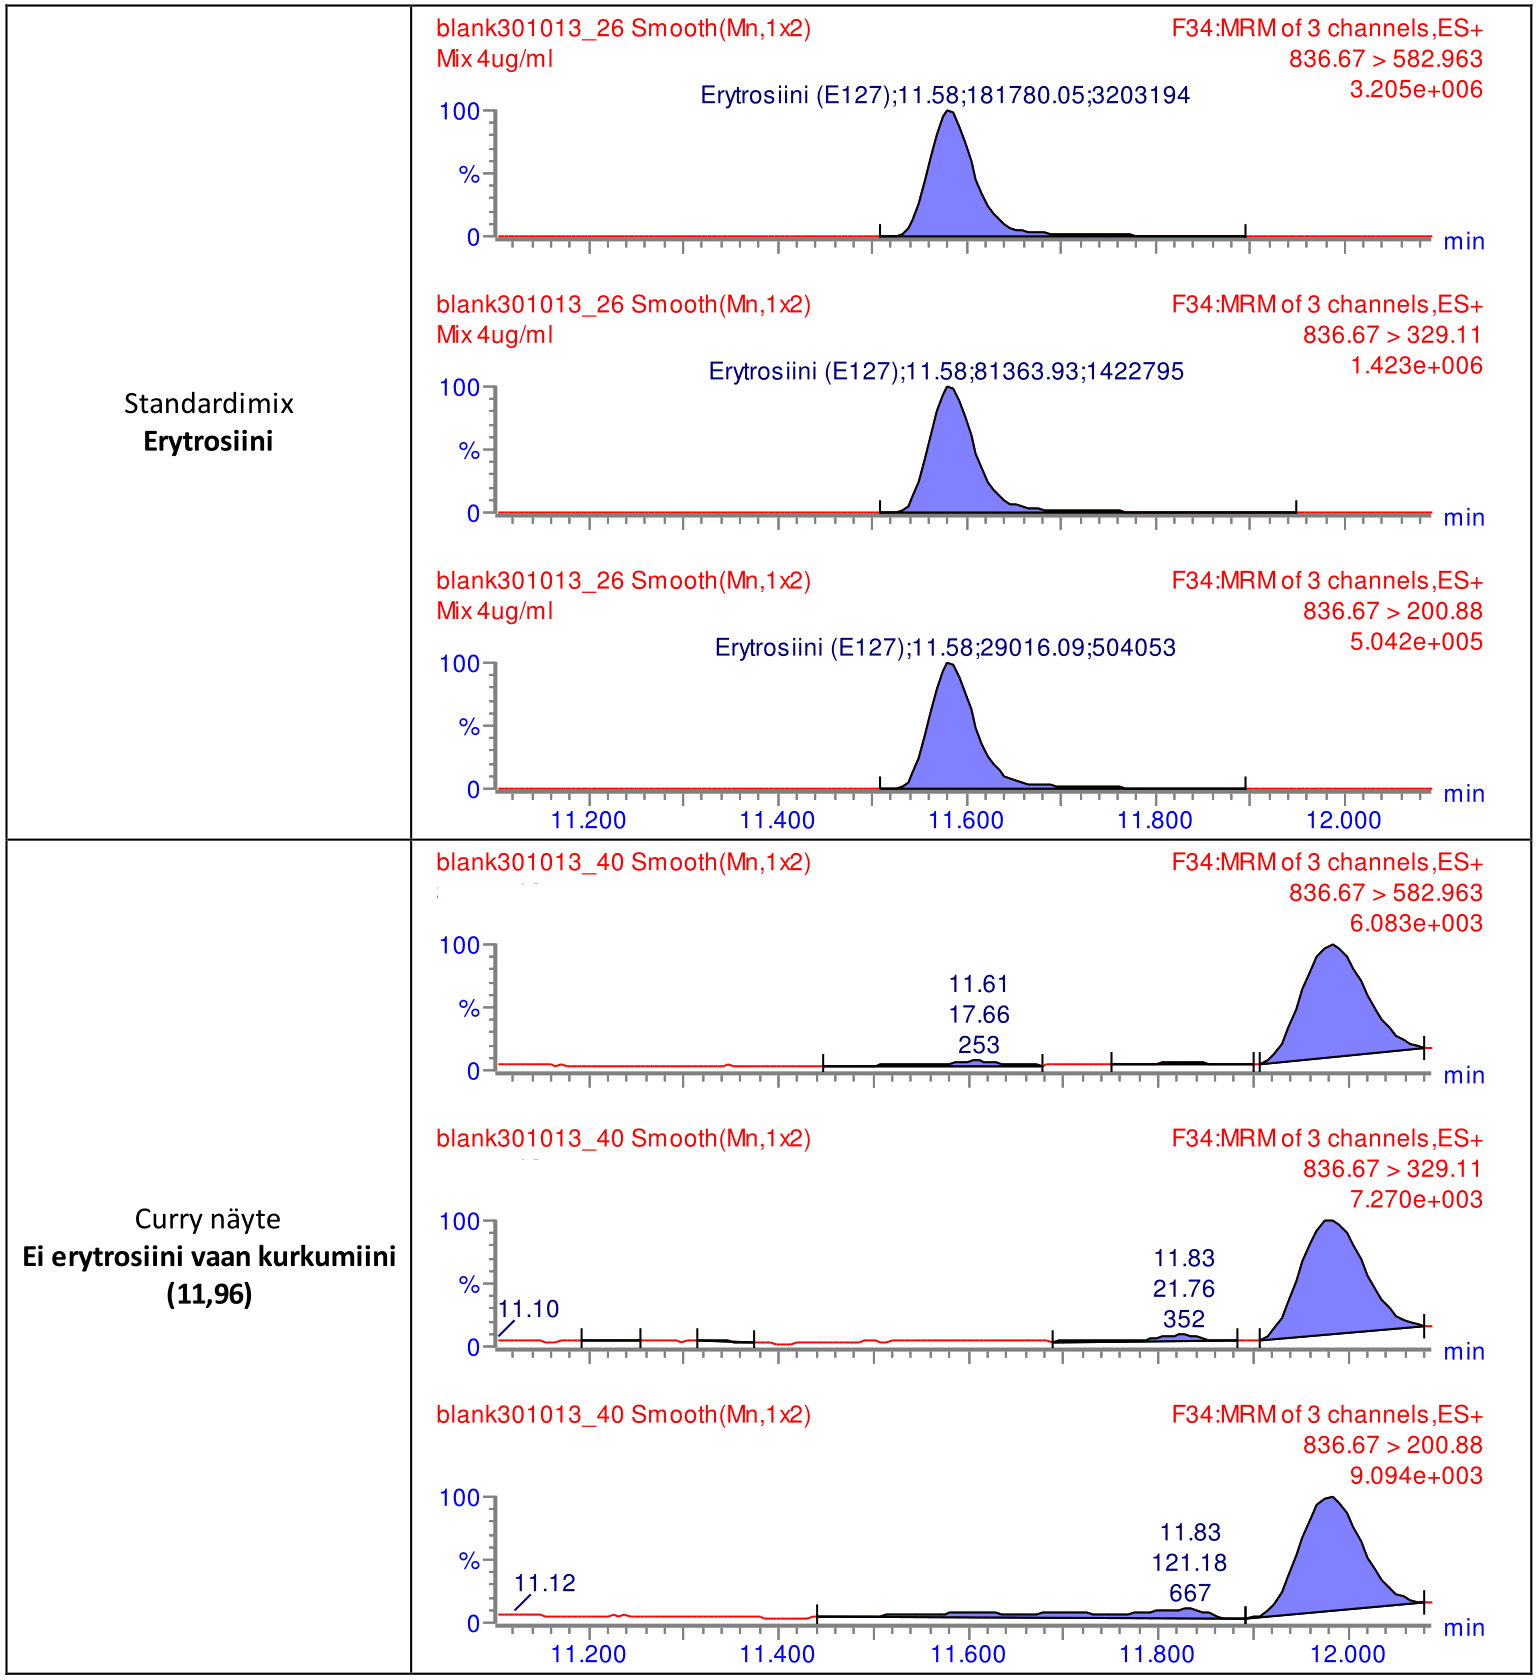
\includegraphics[width=\textwidth]{info-08}
\end{figure}
\begin{figure}[!ht]
  \centering
    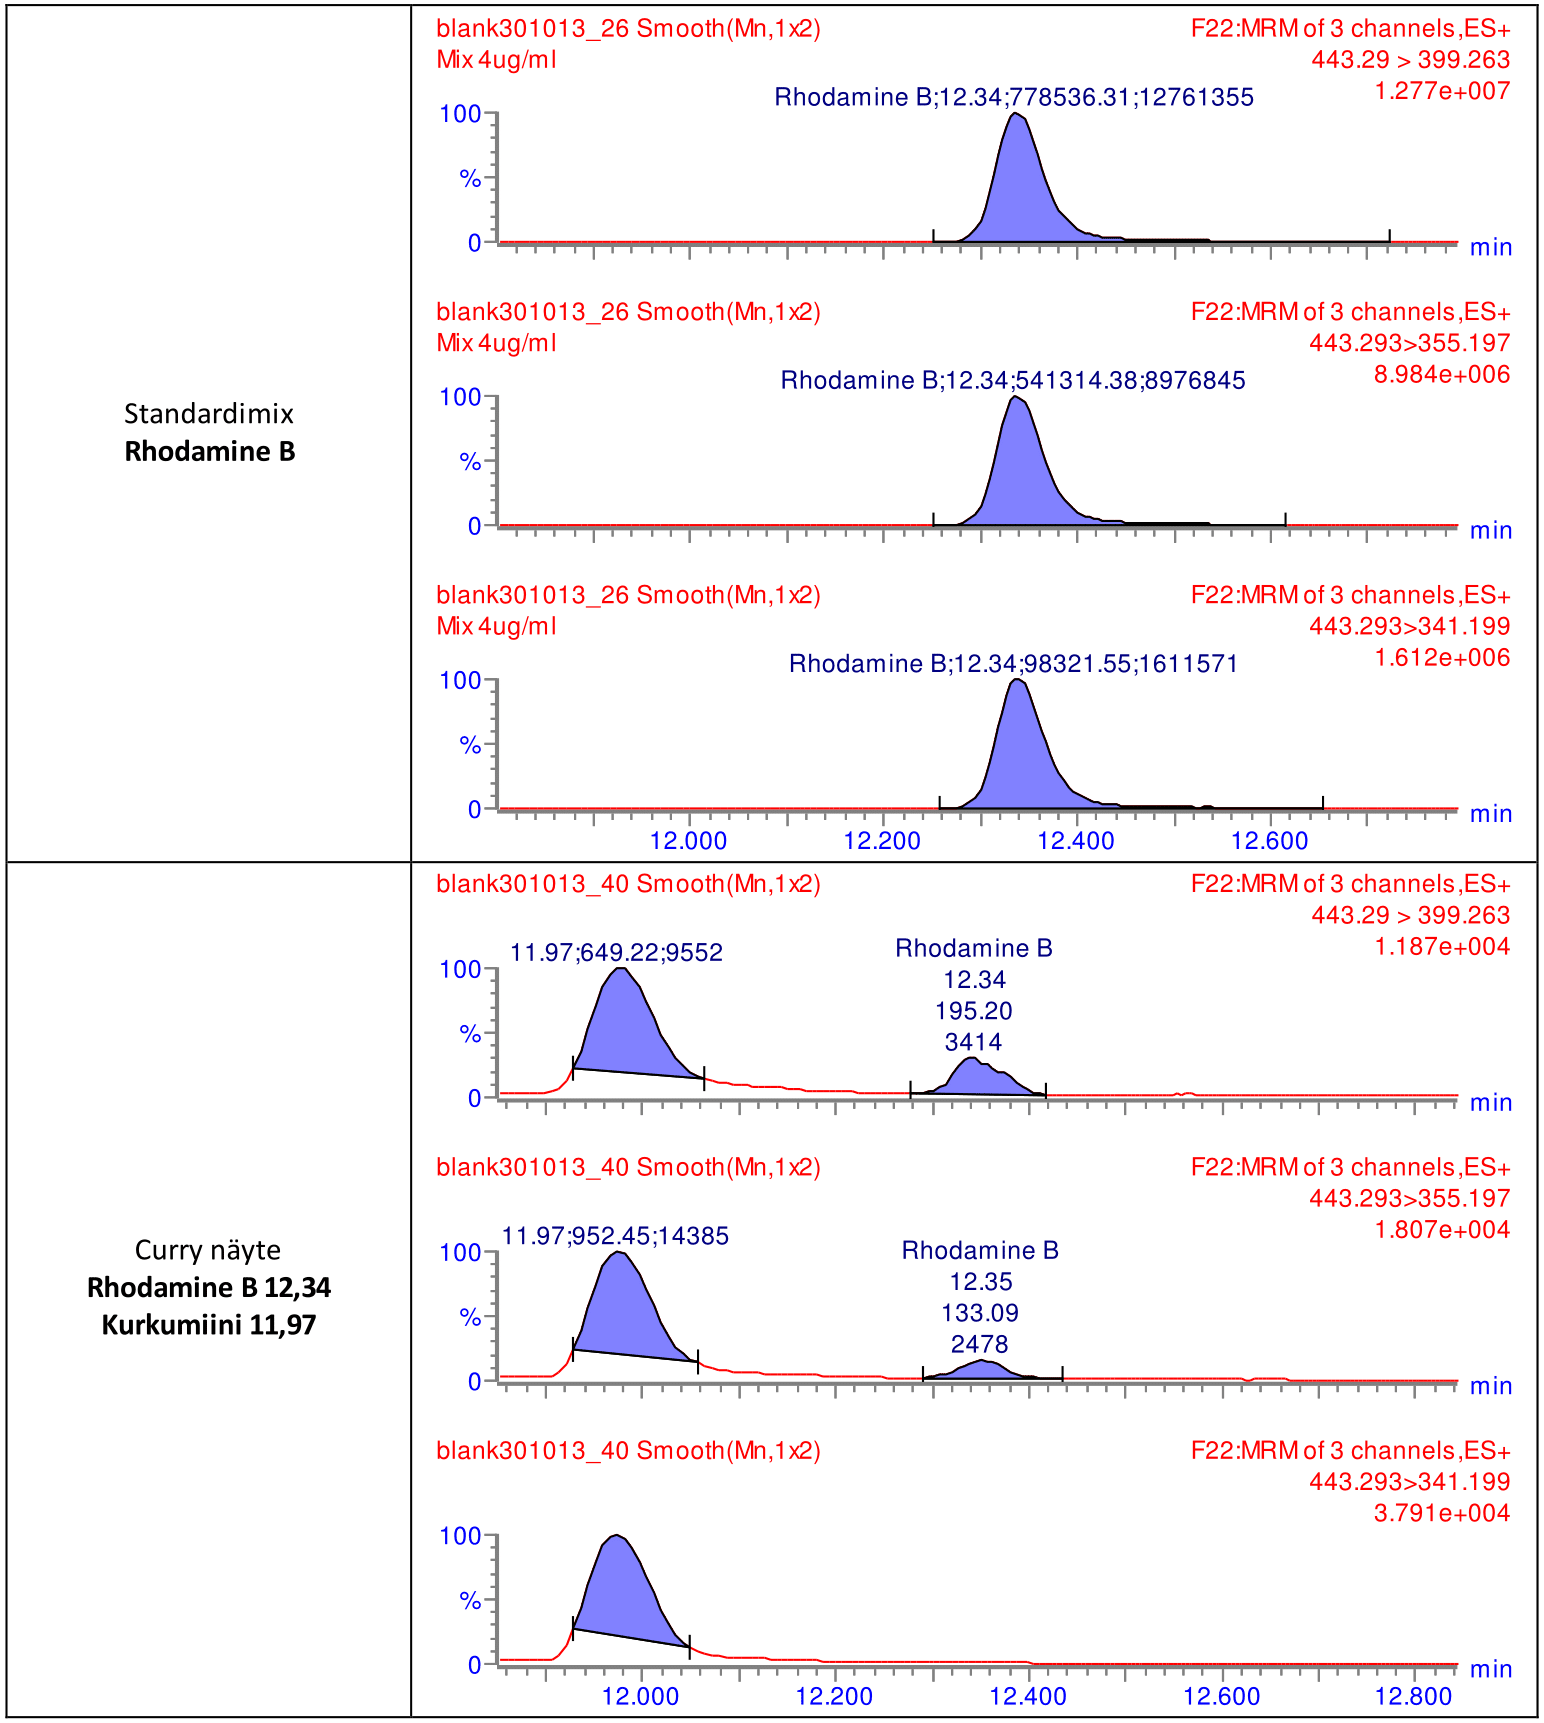
\includegraphics[width=\textwidth]{info-09}
\end{figure}
\restoregeometry
